\documentclass[12pt]{article}
\usepackage{graphicx}
\usepackage{xcolor}
\usepackage[bookmarksnumbered=true]{hyperref} 
\hypersetup{
     colorlinks = true,
     linkcolor = red,
     anchorcolor = blue,
     citecolor = blue
     }
\usepackage{algpseudocode}
\usepackage{textcomp}

\usepackage{caption}
\usepackage{atbegshi}
\usepackage{textcomp}
\usepackage{csquotes}
\usepackage{algorithm}
\algdef{SE}{Begin}{End}{\textbf{begin}}{\textbf{end}}
\usepackage{etoolbox}
\usepackage{cite}
\usepackage{float}
\usepackage{gensymb}
\usepackage{mathtools}
\DeclarePairedDelimiter{\ceil}{\lceil}{\rceil}
\usepackage{cite}
\usepackage{amsmath,amssymb,amsfonts}
\usepackage{textcomp}
\usepackage{xcolor}
\usepackage{multirow}
\usepackage{booktabs}
\usepackage{array}
\usepackage{commath}
\usepackage{adjustbox}



\title{\vspace{-3.0cm}
\centering

\includegraphics[width=4cm,height=4cm,keepaspectratio]{du.jpg} \\ \huge AI Lab Final Report\\ \vspace{0.5cm} \Large \textbf{\textit{Paper Title:}} \textit{On the Completeness of Best-First Search Variants
That Use Random Exploration}\\}


\author{
		\textbf{Submitted By:}\\
        Amit Sarker\\
        Roll: 99\\
                Department of Computer Science and Engineering\\
        University of Dhaka\\
            \and
        \\\textbf{Submitted To:}\\ Dr. Md. Mosaddek Khan \\
        Lecturer\\
        Department of Computer Science and Engineering\\
        University of Dhaka\\\Large \&\\        	
        Md. Mofijul Islam\\
        Lecturer\\
        Department of Computer Science and Engineering\\
        University of Dhaka
}
\date{\today}


\begin{document}
\maketitle

\newpage

\section{Problem Description}
Greedy Best First Search (GBFS) is a popular suboptimal algorithm for solving search problems. GBFS uses a greedy approach to explore a state space, which always gives priority to a node with the lowest heuristic value regardless of cost of reaching this node. Although this greedy approach can be practical, GBFS can also be misled in an arbitrary manner if heuristics are incorrect. For example, consider the Figure~\ref{fig: 1}. In this graph, all nodes in the left subtree below \textbf{v} down to some depth \textbf{d} have a heuristic value of \textbf{4}. Because GBFS considers only the heuristic when evaluating nodes, the algorithm must exhaustively search the entire subtree (or heuristic plateau) before expanding \textbf{n} and finding \textbf{g}. The more misleading the heuristic (i.e. the larger the plateau), the longer it will take to solve this problem.

\begin{figure}[ht]
		\centering
		{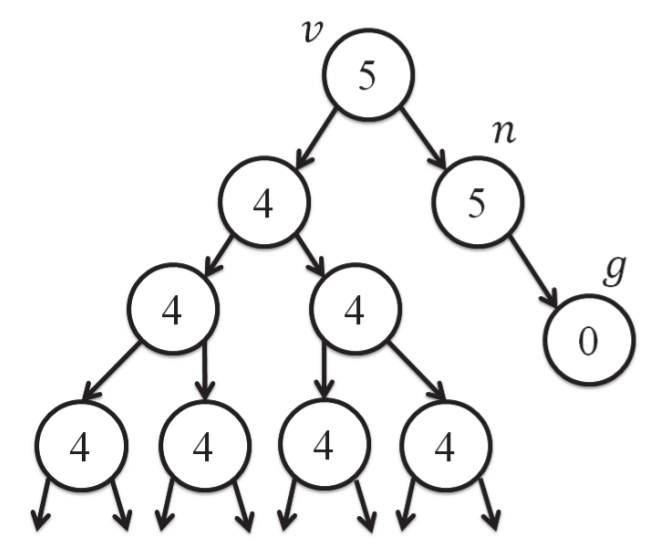
\includegraphics[width=3.0in, height=2.5in]{image1.png}}
		\caption{Graph demonstrating the weaknesses of GBFS.}
        \label{fig: 1}
\end{figure}

\section{Proposed Solution}
Several approaches have enhanced GBFS through the random exploration to preserve the advantages of greediness, while strengthening the algorithm to heuristic error. \textbf{$\epsilon$-greedy node selection} is one of them. These techniques work to encourage the search to ignore the heuristic advice from time to time. On every iteration of a GBFS that uses this technique, the algorithm will expand the node with the lowest heuristic value with probability \textbf{(1 - $\epsilon$)}, where \textbf{$\epsilon$} is a parameter such that 0 $\leq$ $\epsilon$ $\leq$ 1. Otherwise a node is randomly selected from those in the \textit{open list} to expand. Because the resulting algorithm is still greedy for a fraction (1 - $\epsilon$) of the time, the search will still benefit from the value of greediness and quickly pass through areas of the state-space.


\section{Performance Evaluation \& Results}
In this paper, they did not perform any particular performance evaluation for their algorithm. They only gave the proof of the completeness of their proposed \textit{Open-Closed List (OCL)} algorithm for finite graphs. For infinite graphs, they have proved that, the probability that a solution has been found can be made arbitrarily close to \textbf{1} given enough time. But I have done some performance evaluations of their proposed \textbf{OCL} algorithm with the standard \textbf{A* Search} algorithm and \textbf{Best-First search} algorithm based on \textit{total number of nodes vs run time} as well as \textit{total number of nodes vs total number of expanded nodes}. I have considered both finite and infinite (like Figure~\ref{fig: 1}) graphs. Figure~\ref{fig: 2} and Figure~\ref{fig: 3} shows the comparison based on number of nodes vs run time for finite graphs. I have taken the average of 200 iterations to calculate the average run time for all the cases.\\

\hspace*{0.5cm}$\bullet$ \textit{\textbf{Number of nodes vs Run time for finite graphs:}}
\begin{figure}[ht]
		{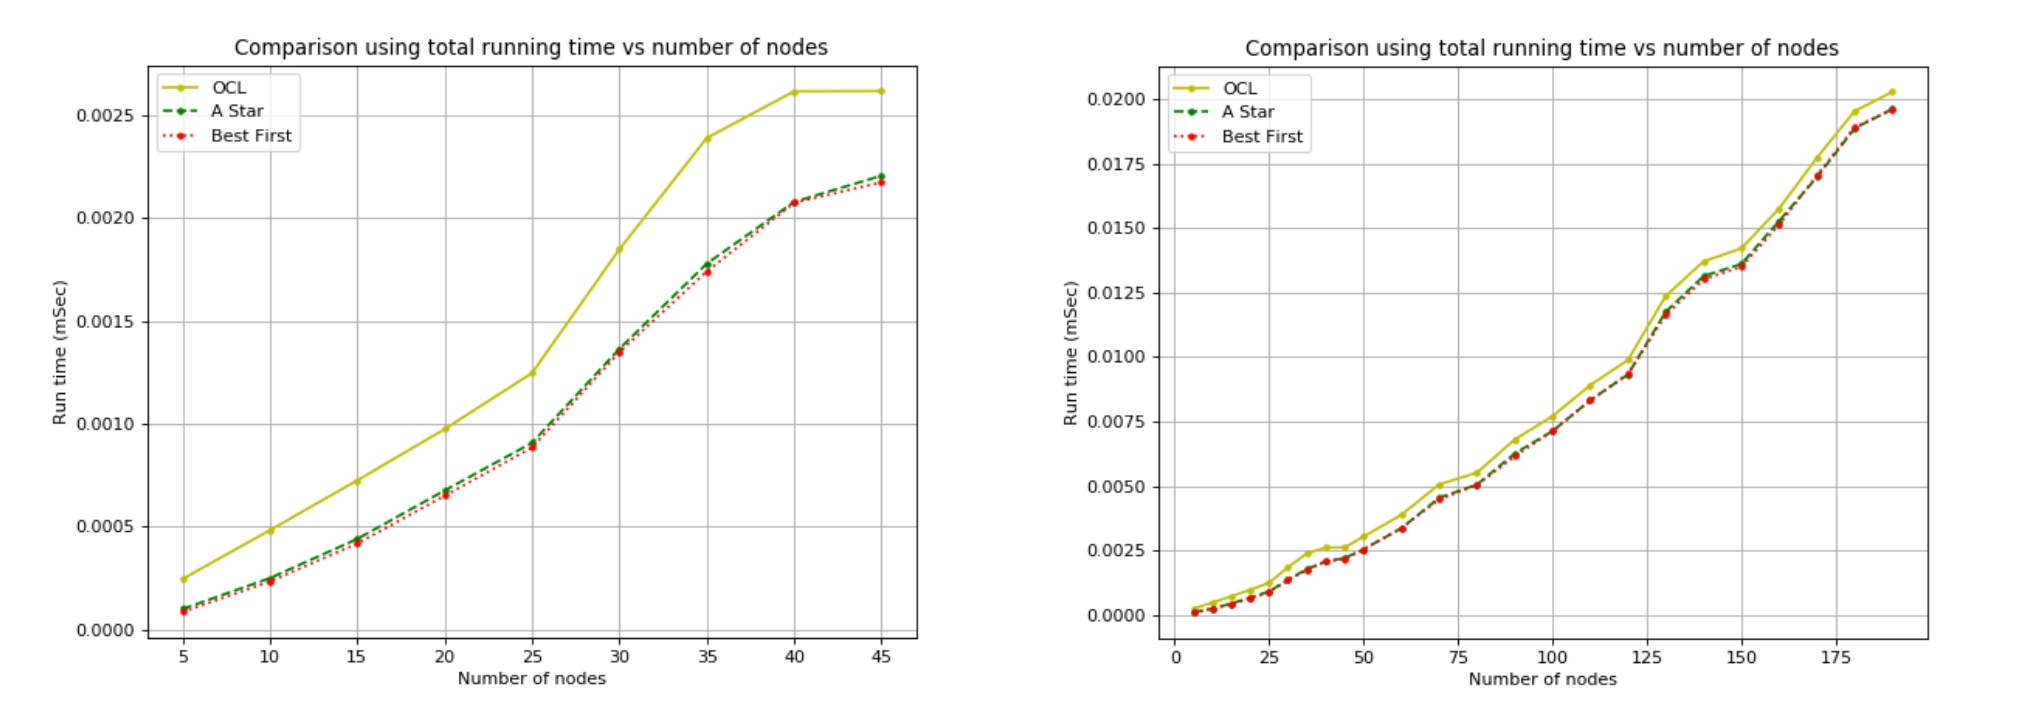
\includegraphics[width=\textwidth,height=2in]{1.jpeg}}
		\caption{Number of Nodes vs Run-time for finite graphs}
        \label{fig: 2}
\end{figure}

\newpage

\begin{figure}[ht]
		{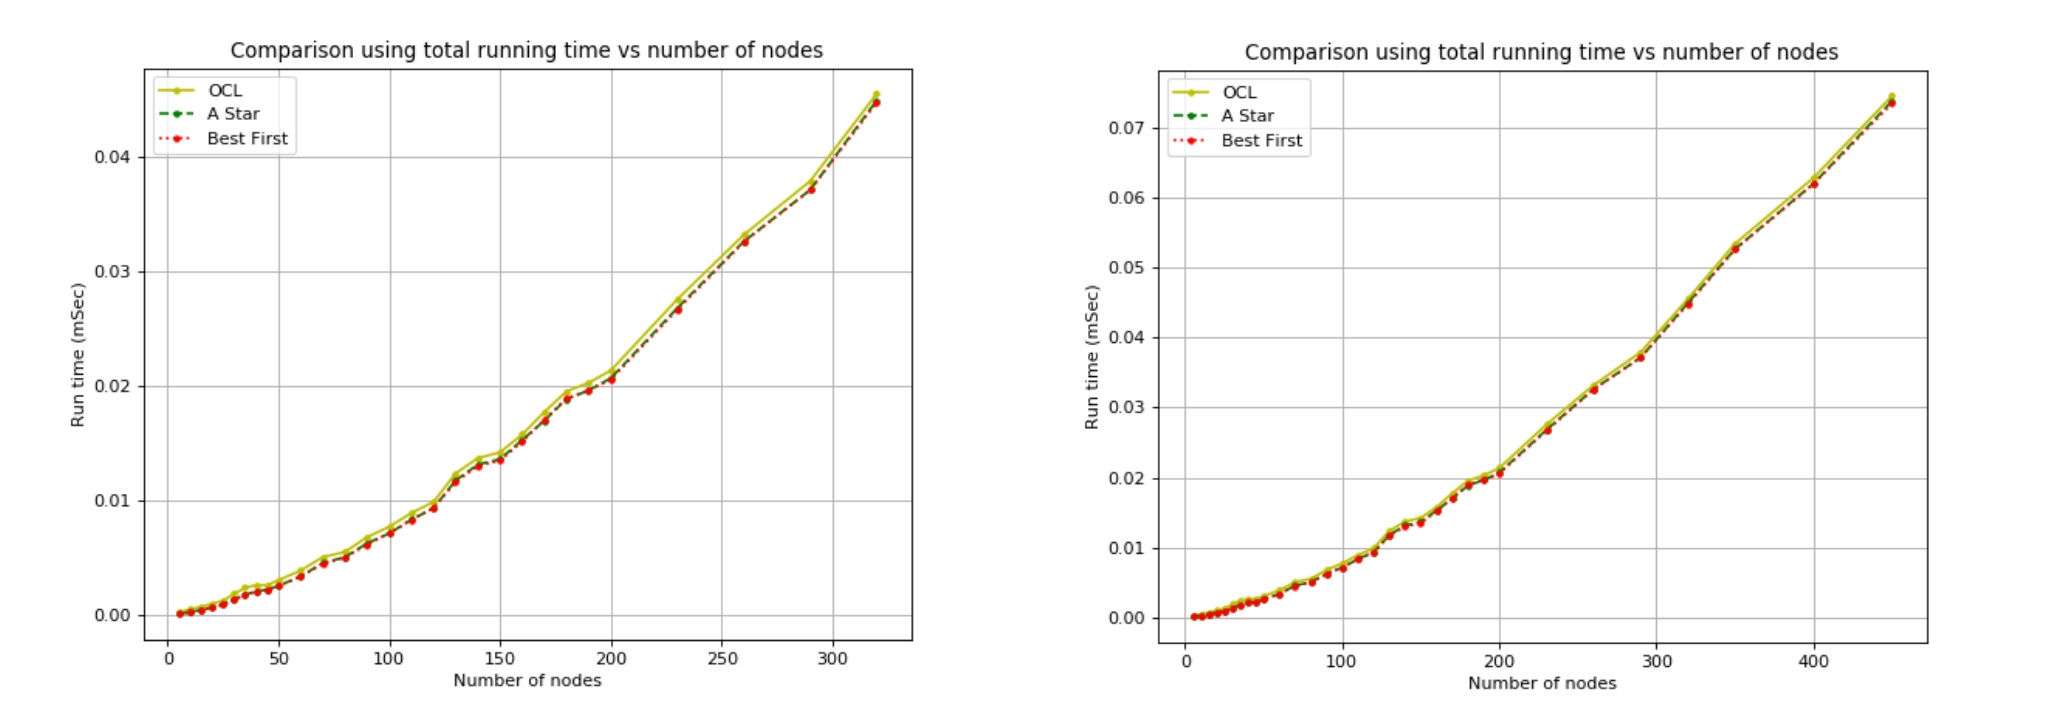
\includegraphics[width=\textwidth,height=2in]{2.jpeg}}
		\caption{Number of Nodes vs Run-time for finite graphs}
        \label{fig: 3}
\end{figure}

From Figure~\ref{fig: 2} and Figure~\ref{fig: 3}, we can see that, their proposed OCL algorithm does not perform better than the standard A* and Best-First search for finite graphs when total number of nodes of the grap are small. When number of nodes are large, OCL performs like standard A* and Best-First search algorithm. The algorithm is complete as it can find the solution whenever solution is available like the standard algorithms. Which supports their claims on finite graphs. They have claimed that, on finite graphs, their proposed algorithm is complete. But they have not claimed anything about the performance of their algorithm for finite graphs.\\

\hspace*{0.5cm}$\bullet$ \textit{\textbf{Number of nodes vs Number of expanded node during search for finite graphs:}}
\begin{figure}[ht]
		{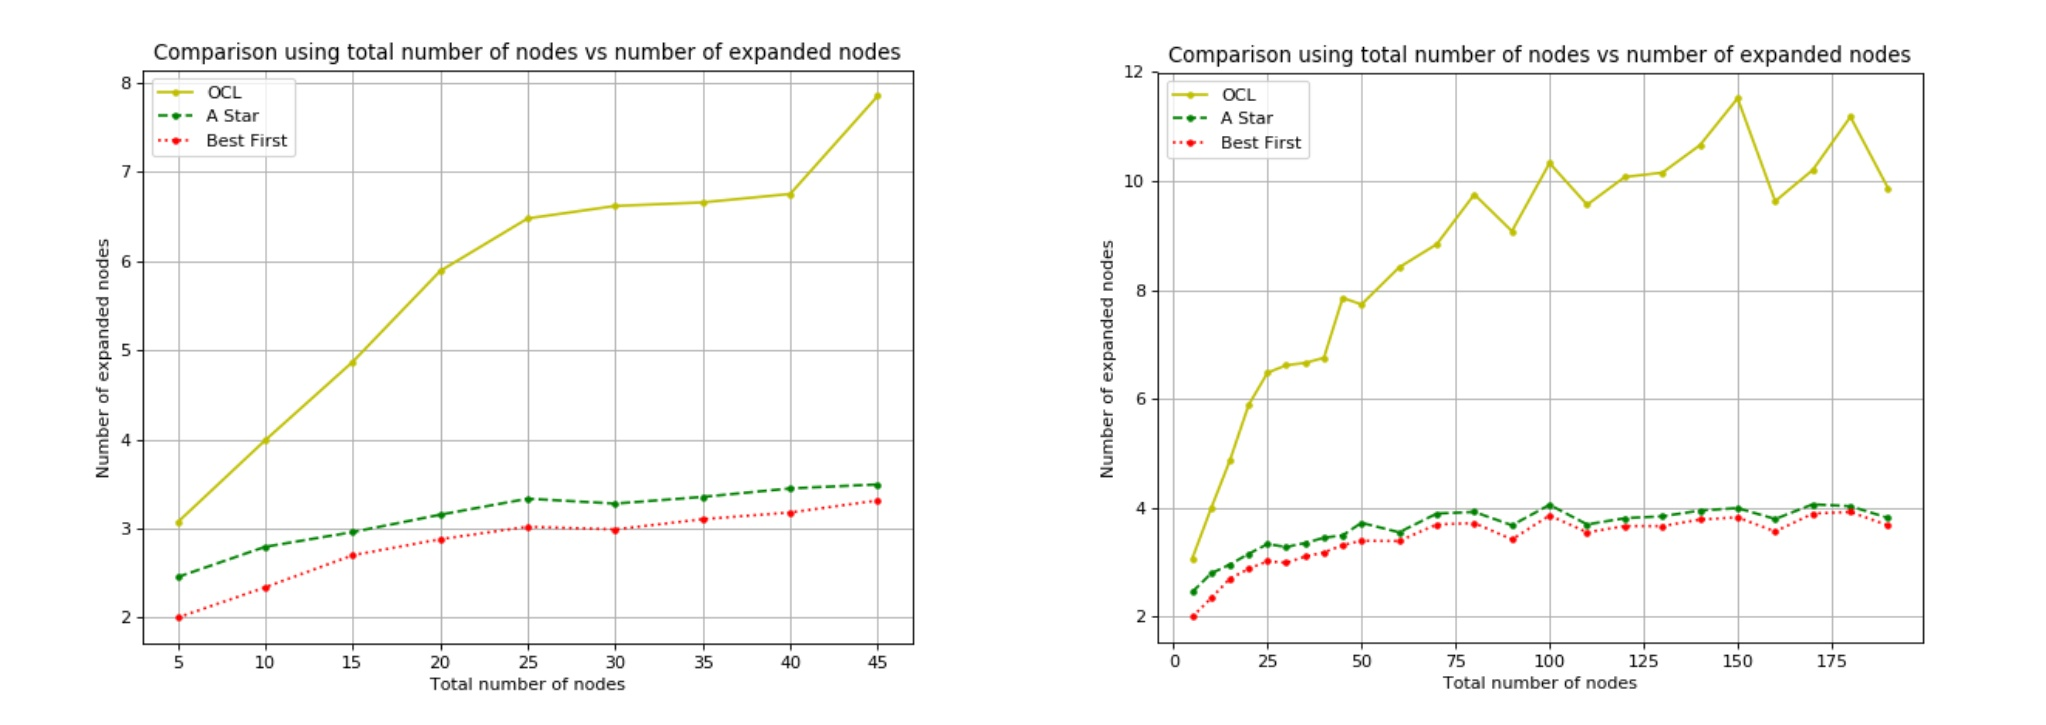
\includegraphics[width=\textwidth,height=2in]{3.jpeg}}
		\caption{Number of Nodes vs Number of expanded nodes for finite graphs}
        \label{fig: 4}
\end{figure}

\newpage

\begin{figure}[ht]
		{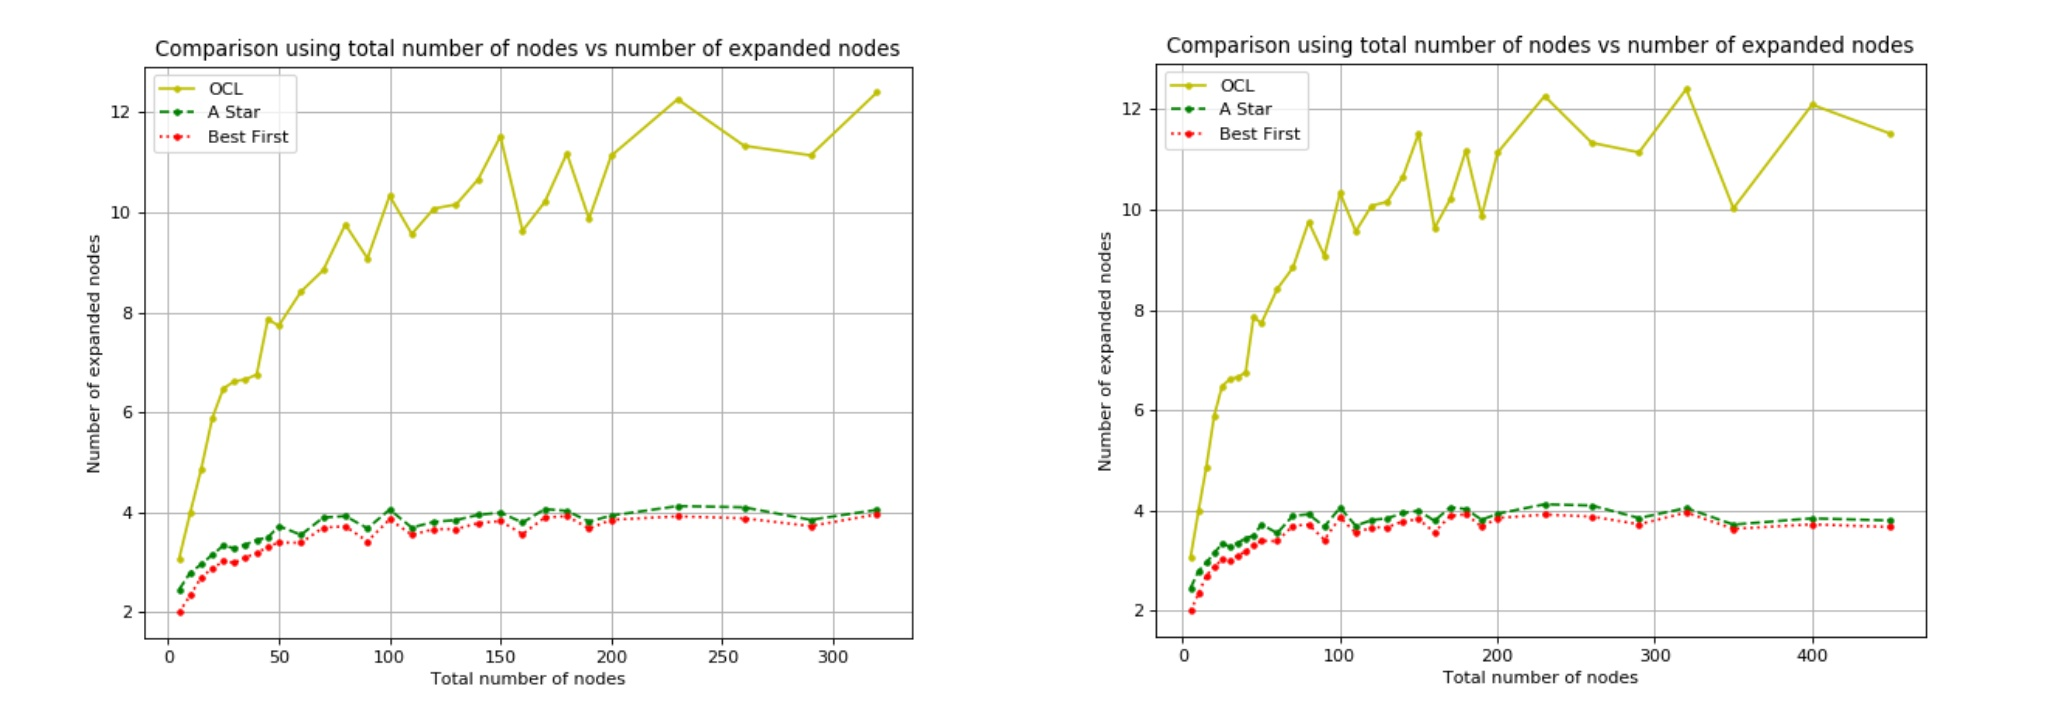
\includegraphics[width=\textwidth,height=2in]{4.jpeg}}
		\caption{Number of Nodes vs Number of expanded nodes for finite graphs}
        \label{fig: 5}
\end{figure}

Figure~\ref{fig: 4} and Figure~\ref{fig: 5} shows that, higher number of nodes are expanded during search in OCL algorithm than that of the standard algorithms for finite graph. So, for finite graphs, OCL does not perform better than the standard A* and Best-First search algorithm.\\

\hspace*{0.5cm}$\bullet$ \textit{\textbf{Number of nodes vs Number of expanded node during search for infinite graphs:}}

\begin{figure}[ht]
		\centering
		{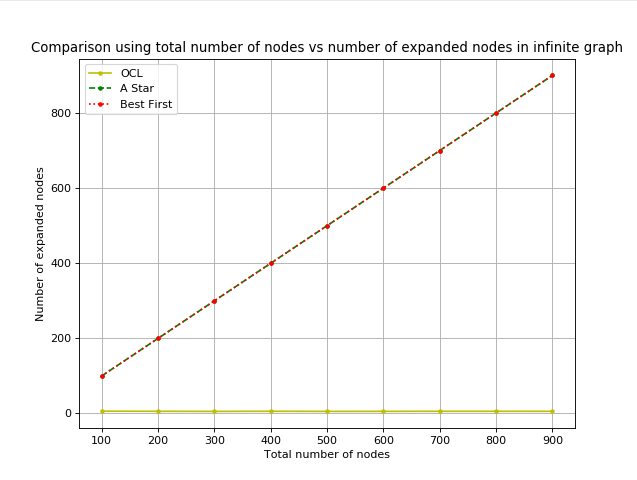
\includegraphics[width=5.0in,height=2.8125in]{inf_1.png}}
		\caption{Number of Nodes vs Number of expanded nodes for infinite graphs}
        \label{fig: 6}
\end{figure}

Figure~\ref{fig: 6} shows the actual strength of OCL algorithm. For infinite graphs (Figure~\ref{fig: 1}), OCL outperforms standard A* and Best-First search algorithms with a huge margin. We can see from the figure that, total number of expanded nodes are proportional to total number of nodes for standard algorithm. But for OCL, only a few number of nodes are needed to be expanded if the graph is infinite. Because for standard algorithms, if the heuristic is misleading, a large number of nodes will be expanded before reaching the goal node. But as OCL uses a stochastic method to expand the next node, only a few nodes will be expanded.

\section{Summary}
Table~\ref{tab: 1} and Table~\ref{tab: 2} summarizes the comparisons based on number of nodes, run time and number of expanded nodes for finite graphs. Table~\ref{tab: 3} summarizes the comparison for infinite graphs. From Table~\ref{tab: 3}, we can say that, OCL outperforms the standard search algorithms for infinite graph which supports the author's claim.

\begin{table}[ht]
\centering
\begin{tabular}{|c|c|c|c|}
\hline
\multirow{2}{*}{Number of Nodes} & \multicolumn{3}{c|}{Run-Time (mSec)} \\ \cline{2-4} 
 & OCL & A* Search & Best-First Search \\ \hline
45 & 0.0027 & 0.0023 & 0.0022 \\ \hline
195 & 0.0205 & 0.0195 & 0.0195 \\ \hline
325 & 0.048 & 0.047 & 0.047 \\ \hline
475 & 0.076 & 0.074 & 0.074 \\ \hline
\end{tabular}
\caption{Comparison of Nodes and Run-Time for finite graphs}
\label{tab: 1}
\end{table}


\begin{table}[ht]
\centering
\begin{tabular}{|c|c|c|c|}
\hline
\multirow{2}{*}{Number of Nodes} & \multicolumn{3}{c|}{\begin{tabular}[c]{@{}c@{}}Number of Expanded Nodes\\ (avg)\end{tabular}} \\ \cline{2-4} 
 & OCL & A* Search & Best-First Search \\ \hline
45 & 8 & 4 & 3 \\ \hline
195 & 10 & 4 & 4 \\ \hline
325 & 12 & 4 & 4 \\ \hline
475 & 12 & 4 & 4 \\ \hline
\end{tabular}
\caption{Comparison of Nodes and Expanded Nodes for finite graphs}
\label{tab: 2}
\end{table}

\newpage

\begin{table}[ht]
\centering
\begin{tabular}{|c|c|c|c|}
\hline
\multirow{2}{*}{Number of Nodes} & \multicolumn{3}{c|}{\begin{tabular}[c]{@{}c@{}}Number of Expanded Nodes\\ (For Infinite Graphs)\end{tabular}} \\ \cline{2-4} 
 & OCL & A* Search & Best-First Search \\ \hline
100 & 5 & 98 & 97 \\ \hline
350 & 6 & 349 & 349 \\ \hline
600 & 6 & 600 & 599 \\ \hline
900 & 6 & 900 & 900 \\ \hline
\end{tabular}
\caption{Comparison of Nodes and Expanded Nodes for infinite graphs}
\label{tab: 3}
\end{table}

\section{Conclusion}
In this paper they have considered the conduct of the best first search algorithms on infinite graphs based on several explorations. In particular, they have shown that, given enough time, it is arbitrarily likely that OCL algorithms can find a solution on the infinite graphs. This result will hold regardless of the accuracy of the heuristic information used. But for finite graph, for small number of nodes, standard algorithms are better than OCL and for large number of nodes, performance of OCL is very close to the standard algorithms.\\\\\\\\
\textbf{Link of the original paper:} \href{http://tinyurl.com/last-choice-ai}{On the Completeness of Best-First Search Variants That Use Random Exploration}



\end{document}